\documentclass[12pt]{article}

\usepackage[margin=1in]{geometry}
\usepackage{graphicx}

% TODO Perform four experiments
%      -  SQT / Perc
%      -  SQT / MA
%      -  MS / Perc
%      -  MS / MA
% TODO put linespoints and move legend in figure 2
% TODO can MA be run on SQT files?

\title{Rapid and accurate peptide identification from tandem mass
  spectra}

\author{Christopher Y. Park \\
Department of Genome Sciences\\
University of Washington\\
Seattle, WA, USA
\and
Aaron A. Klammer\\
Department of Genome Sciences\\
University of Washington\\
Seattle, WA, USA
\and
Lukas K\"{a}ll\\
Department of Genome Sciences\\
University of Washington\\
Seattle, WA, USA
\and
William S. Noble\footnote{To whom correspondence should
  be addressed}\\
Department of Genome Sciences\\
Department of Computer Science and Engineering\\
University of Washington\\
Seattle, WA, USA
}

\begin{document}

\maketitle

\begin{abstract}
Mass spectrometry, the core technology in the field of proteomics,
promises to enable scientists to identify and quantify the entire
complement of proteins in a complex biological sample.  Currently, the
primary bottleneck in this type of experiment is computational.
Existing algorithms for interpreting mass spectra are slow and fail to
identify a large proportion of the given spectra.

We describe a database search program called Crux that extends the
state of the art in peptide identification in several significant
respects.  Crux reimplements and extends the widely used database
search program {\sc Sequest}.  For speed, Crux uses a peptide indexing
scheme to rapidly retrieve candidate peptides for a given spectrum.
For each peptide in the target database, Crux generates shuffled decoy
peptides on the fly, providing a good null model and, hence, accurate
false discovery rate estimates.  Crux also implements two recently
described postprocessing methods: a $p$~value calculation based upon
fitting a Weibull distribution to the observed scores, and a
semi-supervised method that learns to discriminate between target and
decoy matches.  Both methods significantly improve the overall rate of
peptide identification.
\end{abstract}

\section{Introduction}

Tandem mass spectrometry is the method of choice for many protein
identification studies.  However, this technology suffers from an
analysis bottleneck, with a need for more efficient and more accurate
methods of mapping from the observed fragmentation spectra to the
corresponding peptides.

The most widely used methods for peptide identification, such as
{\sc Sequest} \cite{eng:approach}, MASCOT \cite{perkins:probability},
X!Tandem \cite{craig:tandem} and Inspect \cite{tanner:inspect},
exploit a database of known protein sequences.  For each observed
spectrum, these methods search the database for the peptide whose
theoretical spectrum best matches the observed spectrum.  The
resulting peptide-spectrum matches (PSMs) can be ranked using a
pre-defined score function, or by using machine learning methods such
as linear discriminant analysis \cite{keller:empirical}, support
vector machines \cite{anderson:new, kall:semi-supervised} or decision
trees \cite{elias:intensity}.

\begin{figure*}
\centering
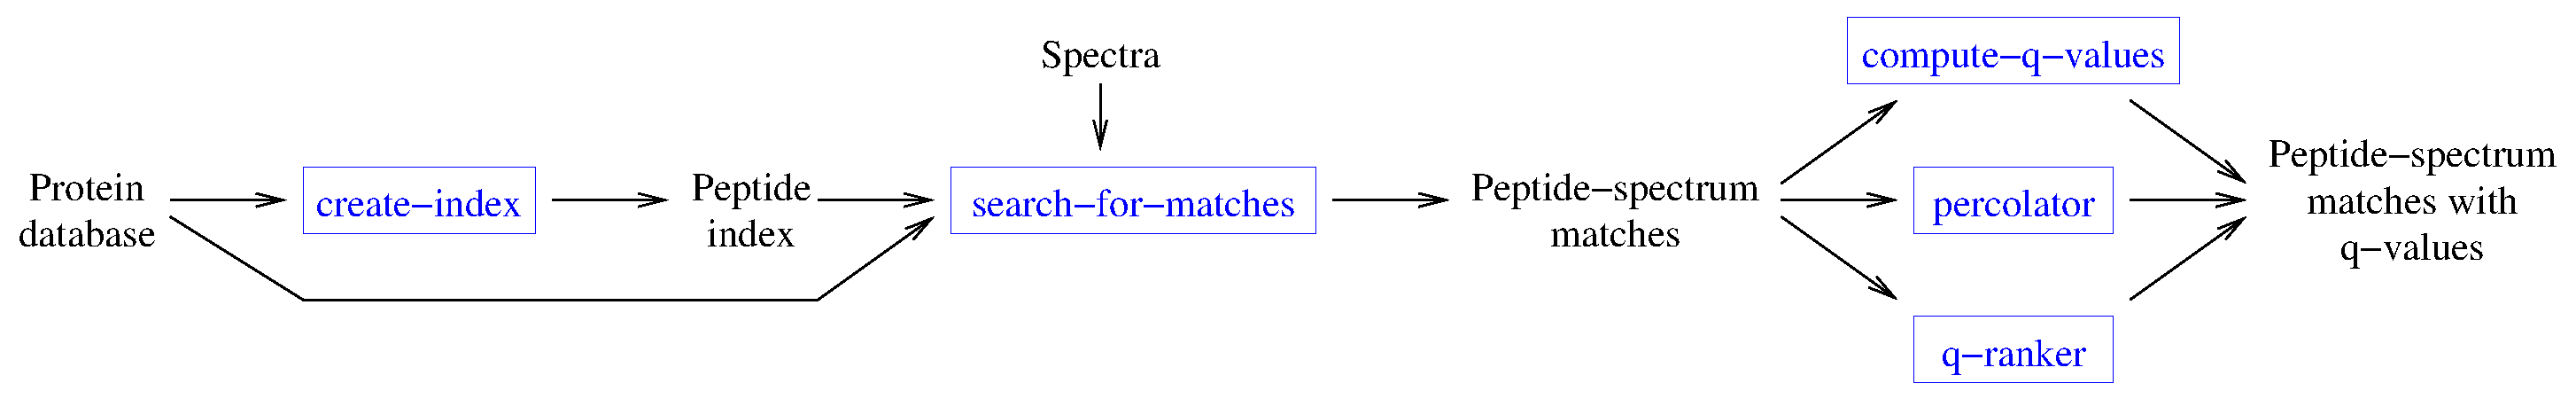
\includegraphics[width=6.5in]{schematic.eps}
\caption{{\bf The Crux algorithm.}  Crux takes as input a collection
  of fragmentation spectra and a target protein sequence database, and
  produces a list of peptide-spectrum matches, each with an associated
  $q$~value.
  \label{figure:crux}}
\end{figure*}

In this work, we describe a computational tool called Crux that solves
the peptide identification problem efficiently and accurately.  
Figure~\ref{figure:crux} is a schematic diagram of Crux's workflow.


, Crux incorporates a rapid
peptide lookup scheme, a static scoring system for relative ranking of
peptides with respect to each spectrum, on-the-fly generation of decoy
peptides, two alternative post-processing methods to re-rank the PSMs,
and modules to compute the statistical significance of of each PSM.
Relative to the current state of the art, Crux makes the following
primary contributions:

\begin{itemize}

\item {\bf Efficient retrieval of candidate peptides.}  Given a
  spectrum with a specified precursor mass-to-charge ratio (m/z), Crux
  uses a precomputed peptide database to retrieve efficiently all
  peptides whose m/z lies within a user-specified window around the
  target m/z (called {\em candidate peptides}).  The database is
  sorted by peptide mass and is stored on disk, with mass indices
  stored in memory.  We show that, relative to {\sc Sequest}'s strategy of
  reading the protein sequence database from disk for each new
  spectrum, the indexed database decreases search time by X\% on
  average.

\item {\bf On-the-fly generation of decoy peptides.}  In evaluating
  the statistical significance of a PSM, mass spectrometrists
  frequently employ a {\em decoy database} comprised of protein
  sequences that have been reversed, shuffled or generated from a
  Markov chain derived from the given {\em target database}.  The
  number of matches to the decoy database yields an estimate of the
  false discovery rate associated with a collection of target PSMs.
  Crux uses this target-decoy strategy, generating decoys by shuffling
  the target peptides.  This approach ensures that each decoy peptide
  exhibits precisely the same amino acid composition and total mass as
  the corresponding target decoy.  To avoid the memory overhead
  associated with storing shuffled, non-overlapping decoy peptides in
  memory, Crux generates decoy peptides on the fly.

\item {\bf Two state-of-the-art PSM re-ranking algorithms} After
  scoring all peptides with respect to a given spectrum, the
  top-ranked PSM must be ranked with respect to other PSMs from the
  same data set.  Some score functions, such as {\sc Sequest}'s
  cross-correlation score ($XCorr$), have been used to carry out both
  relative ranking and absolute ranking; however, numerous studies
  have demonstrated that better absolute rankings can be achieved by
  using machine learning methods \cite{keller:empirical, anderson:new,
  elias:intensity, kall:semi-supervised}.  Crux incorporates two
  recently described methods for re-ranking PSMs.  The first method,
  called Percolator \cite{kall:semi-supervised}, trains a machine
  learning method to discriminate between target and decoy PSMs.  This
  dynamically trained model incorporates specific characteristics of
  the given data set.  The second method fits the observed $Xcorr$
  scores to a Weibull distribution, and uses the resulting
  distribution to compute accurate $p$~values \cite{klammer:not}.

\item {\bf Accurate false discovery rate estimates.}  Crux uses
  well-established statistical methods to estimate false discovery
  rates based upon decoy PSMs \cite{benjamini:controlling}.  Crux
  reports, along with each PSM, a $q$~value, which is defined as the
  minimal false discovery rate threshold at which a given PSM is
  deemed correct \cite{storey:statistical}.  Depending upon the
  post-processing method, Crux estimates these $q$~values either using
  decoy PSMs or, for the Weibull curve fitting, directly from the
  estimated $p$~values.

\end{itemize}

Perhaps most significantly, from the perspective of the mass
spectrometry research community, Crux provides all of the above in a
single stand-alone C program which is distributed, with source code,
free for academic use.  Below, we demonstrate that Crux is both
efficient and accurate, yielding FIXME.

\section{Results}

\subsection{Efficient retrieval of candidate peptides}

When presented with a new query spectrum and its associated precursor
mass, Crux must first retrieve from the sequence database all of the
candidate peptides, i.e., peptides whose masses lie within a specified
range of the precursor mass.  A straightforward retrieval method is to
read the entire database from disk for each query, evaluating
candidate peptides as they are encountered.  This approach, which is
used by {\sc Sequest}, is space-efficient but can be slow for large
databases.

In addition to implementing the above approach, Crux offers an
alternative strategy that allows for more efficient candidate peptide
retrieval.  In this approach, the user must pre-process a given
protein database to produce a binary protein database and a binary
peptide index.  The pre-processing step sorts all of the peptides in
the database by mass and stores pointers to their locations in the
protein database (sequence index, start position, and peptide length).
Crux can then quickly retrieve a set of candidate peptides via a
simple range query on the peptide index.

Upon execution, Crux accesses the binary protein database and the
peptide index as memory-mapped files.  This approach offloads to the
operating system the decision about how much of the database to store
in memory, ensuring that small databases are read fully into memory
but large databases are paged into and out of memory only as needed.

\begin{figure}
  \centering
  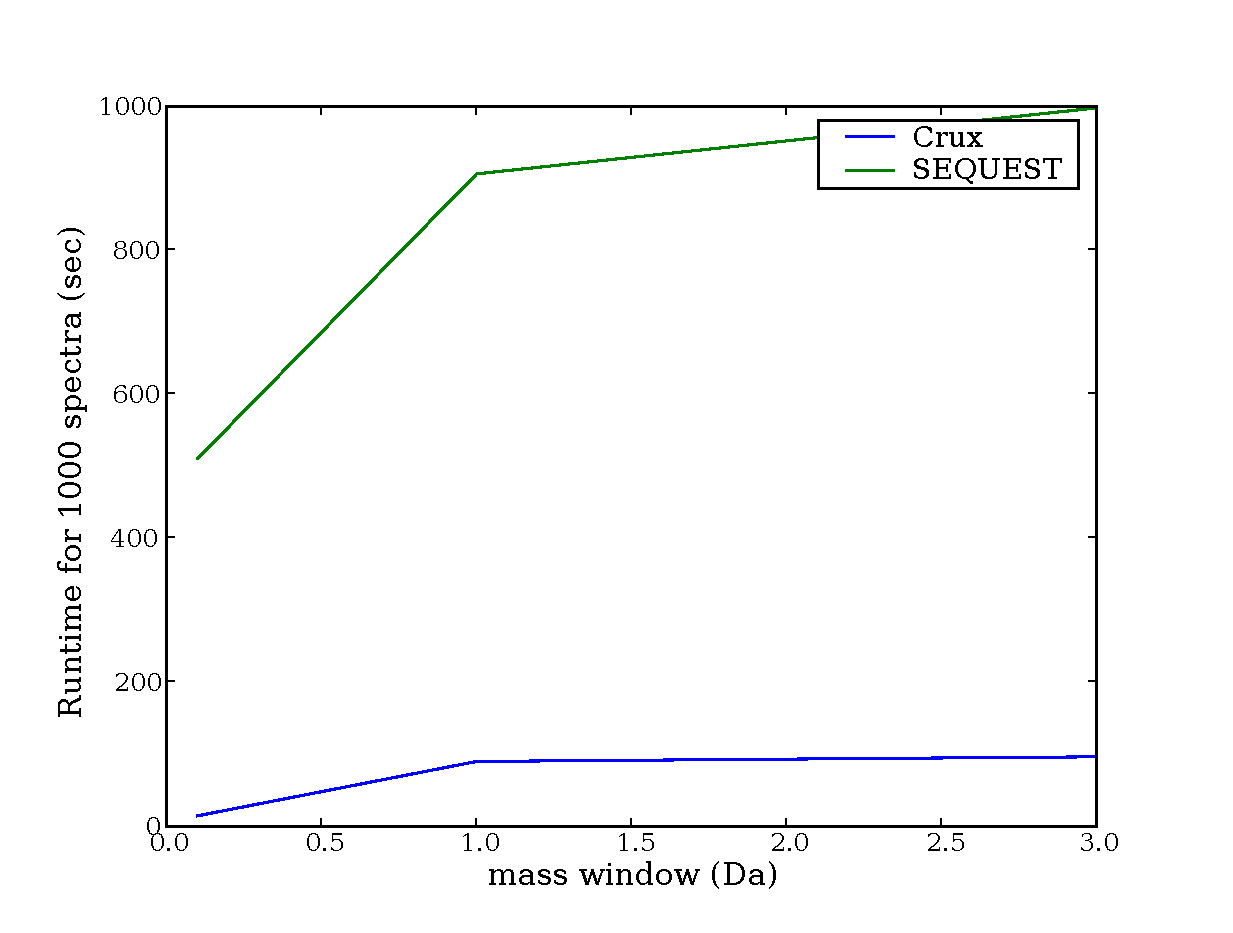
\includegraphics[width=5in]{./Images/indexing.eps}
  \caption{{\bf Rapid database searching.}  The figure plots the total
  running time required to search 1,000 tandem mass spectra against
  the yeast protein database, plotted as a function of the m/z
  tolerance used to define candidate peptides.  The three series
  correspond to searching with {\sc Sequest} and searching with Crux
  with and without a peptide index.  For purposes of comparison,
  Crux's decoy searching and post-processing are turned off.
  \label{figure:indexing}}
\end{figure}

To demonstrate the efficiency of Crux's candidate peptide retrieval
strategy, we searched with a collection of 100 spectra against the
NRDB, generating candidate peptides from a series of increasing wider
m/z windows.  Figure~\ref{figure:indexing} plots the search time as a
function of m/z window width.  For this experiment, we use a modified
version of {\sc Sequest} that only computes Sp (and not XCorr), and we
compare its running time to that of Crux running in the same fashion.
As expected, Crux runs more quickly than {\sc Sequest}, because Crux does
not need to scan the entire database to retrieve a small collection of
candidate peptides.  The difference is most pronounced when the mass
tolerance window is small.  For example, with a mass tolerance window
of 0.1, {\sc Sequest} requires 3.5~hrs clock time, whereas Crux requires
0.1~hrs.  This represents a 35-fold improvement.  However, even when
we use a mass tolerance of 3, Crux yields a six-fold speed improvement
(0.6~hours versus 3.6~hours).

\subsection{Accurate reimplementations of $Sp$ and $Xcorr$}

{\sc Sequest} is the first and one of the most widely used database
search methods for peptide identification from tandem mass spectra.
Crux therefore begins with a reimplementation of the core of {\sc
Sequest}.  After retrieving all of the candidate peptides for a given
spectrum, the candidates are ranked according to the preliminary {\sc
Sequest} score $Sp$.  Subsequently, the 500 top-scoring peptides are
re-ranked according to the cross-correlation score $XCorr$.

For $Sp$ scoring, Crux applies several pre-processing steps to the
observed spectrum.  First, Crux takes the square root of each peak's
intensity and rounds each peak's m/z to the nearest integer.  Second,
Crux normalizes the peak intensities to sum to 100.  Third, Crux
extracts the top 200 highest intensity peaks.  Crux compares the
resulting observed spectrum $v$ with the b and y fragment ions $u$ from the
candidate peptide to compute $Sp$ as follows:
\[
S_p(u, v) = \frac{
\left(\sum_{i=1}^N v_i \delta(u_i) \right)
\left(\sum_{i=1}^N \delta(u_i v_i)\right)
\left(1 + 0.075 R(u, v) \right)
}{\sum_{i=1}^N \delta(u_i)}
\]
where $N$ is the maximal m/z value, $R(u, v)$ is the maximum number of
consecutive b- or y-ions from the theoretical spectrum that appear in
the observed spectrum, and $\delta(x) = 0$ if $x=0$ and $\delta(x) =
1$ otherwise.

$Xcorr$ scoring also requires some pre-processing of the observed
spectrum.  As before, Crux first takes the square root of each peak's
intensity and rounds each peak's m/z to the nearest integer.  Second,
Crux divides the spectrum into 10 regions and normalizes the spectrum
intensity in each region to maximum of 50.0. To create the theoretical
spectrum from the candidate peptide, Crux constructs a spectrum with
peak intensity 50.0 for b and y ions, 25.0 for the $\pm 1$ m/z flanking
peaks of each b and y ion, and 10.0 for ions resulting from a neutral
loss of ammonia from b or y ions or neutral loss of water from b ions.
Crux then computes $Xcorr$ as follows:
\[
X_c(u, v) = \frac{0.015\sum_{i=1}^N u_i v_i}
{\sum_{\tau=-75}^{75} \sum_{i=1}^N u_i v_{i-\tau}}
\]

\begin{figure*}
  \centering
  \begin{tabular}{cc}
    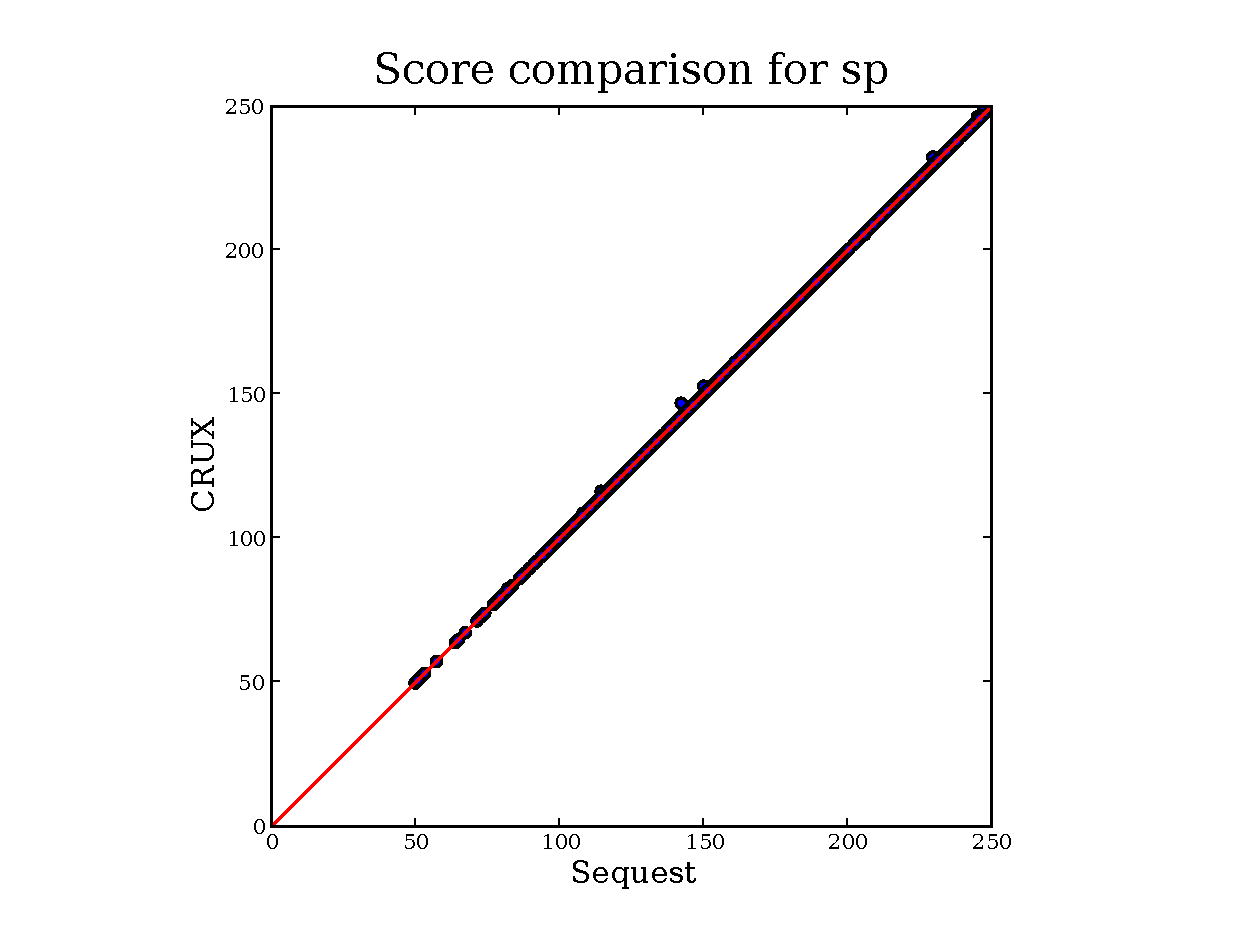
\includegraphics[width=3in]{./Images/random-sp.eps} &
    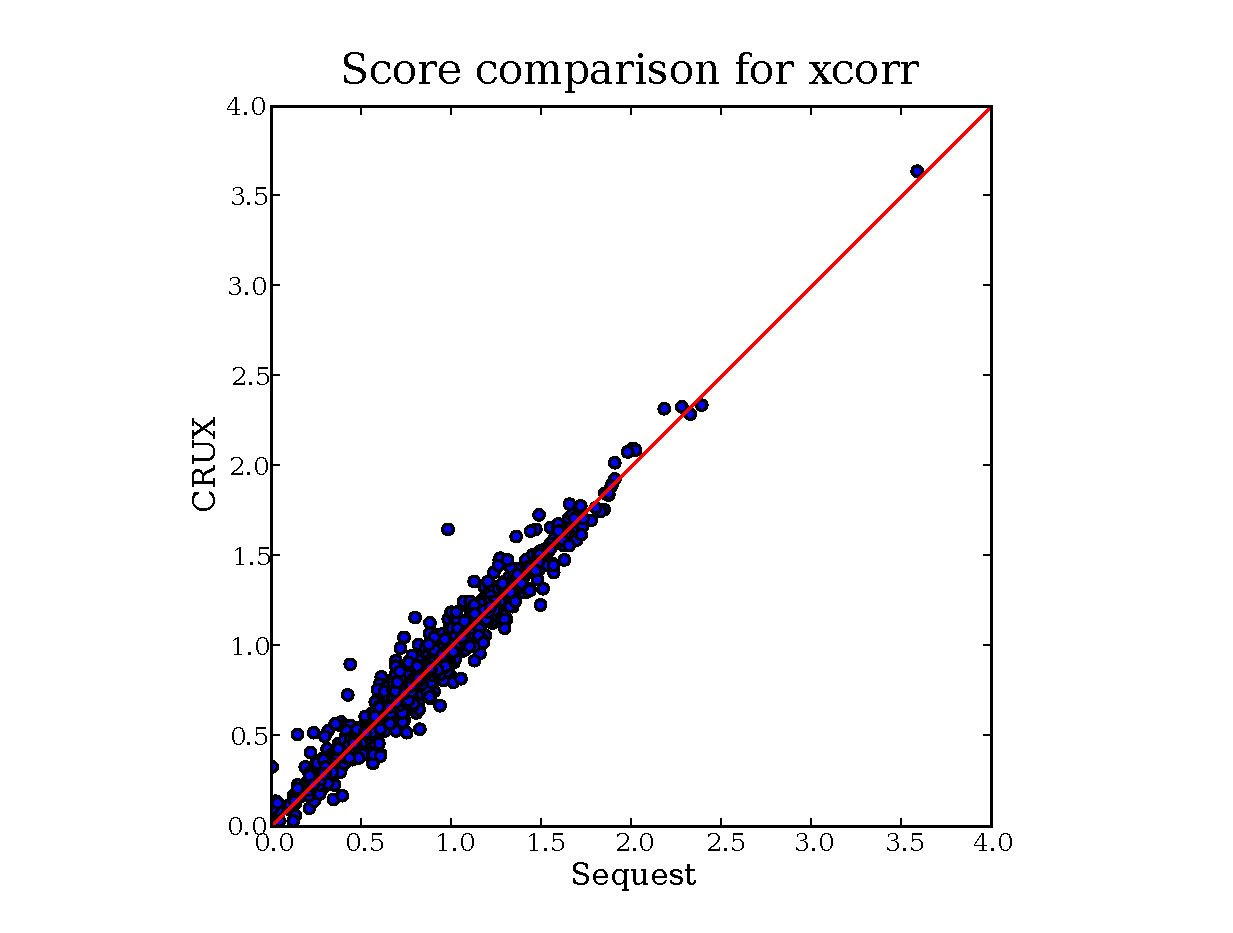
\includegraphics[width=3in]{./Images/random-xcorr.eps} \\
  A & B \\
  \end{tabular}
  \caption{{\bf Re-implementation of Sp and Xcorr scoring functions.}
  The figure plots, for a collection of peptide-spectrum matches, the
  Sp (A) and XCorr (B) scores as computed by Crux as a function of the
  same scores as computed by {\sc Sequest}.
  \label{figure:sp-xcorr}}
\end{figure*}

Figure~\ref{figure:sp-xcorr} shows that the Crux-calculated versions
of $Sp$ and $Xcorr$ closely match the {\sc Sequest}-calculated
versions of these scores.  The vast majority of the PSMs receive
identical scores using either method.  Among a collection of FIXME
spectra, searched with a mass window of FIXME m/z, the top-ranked
peptide according to Crux differs from the top-ranked peptide
according to {\sc Sequest} in only FIXME cases.

\subsection{Null peptide generation}

When identifying peptides from tandem mass spectra, a commonly used
null model is to search the given set of spectra against a {\em decoy
database}.  A decoy database is a database of amino acid sequences
that is derived from the original protein database (called the {\em
target database}) by reversing the target sequences
\cite{moore:qscore}, shuffling the target sequences
\cite{klammer:effects}, or generating the decoy sequences at random
using a Markov model with parameters derived from the target sequences
\cite{colinge:olav}.  Ideally, the decoy database should contain
peptide-like amino acid sequences that are not in the target database.

Crux uses a decoy strategy; however, rather than generating a fixed
decoy database, Crux generates decoys on the fly.  For each comparison
between a spectrum and a target peptide, Crux generates a
corresponding decoy peptide by shuffling the non-terminal amino acids
of the target peptide.  Consequently, Crux reports for every target
PSM one or more corresponding decoy PSMs.  On-the-fly decoy generation
introduces a small computational overhead but saves space, because the
decoy database does not need to be stored.

The primary advantage of generating decoys on the fly is that the
resulting decoys share exactly the same total mass and amino acid
composition as the target.  When using a static decoy database,
ensuring that the target and decoy peptide mass and amino acid
composition stays the same is very difficult.  For example, shuffled
and Markov chain-generated decoy databases will not retain these
properties.  A reversed database will retain these properties, but
only when trypticity is not enforced.  On-the-fly decoy generation has
the further advantage that, unlike reversed decoys, multiple decoys
can be generated for a single target.  These additional decoys can be
useful if the user wants more accurate confidence estimates.

\subsection{Improved identification of peptides}

Identifying peptides from tandem mass spectra via database search is,
fundamentally, a ranking procedure, in which good PSMs are ranked
above poor PSMs.  Furthermore, this ranking task can be usefully
separated into two phases: a {\em relative ranking} task, in which all
of the candidate peptides are ranked relative to a single spectrum to
identify a single best PSM for that spectrum, and an {\em absolute
ranking} task, in which the top-ranked PSMs for multiple spectra are
ranked relative to one another.  Absolute ranking is, by definition,
more difficult than relative ranking.  Furthermore, empirical evidence
suggests that, although $Xcorr$ does a good job at relative ranking,
it performs more poorly when attempting to rank PSMs absolutely
\cite{keller:empirical, anderson:new}. Crux therefore implements two
recently described methods for post-processing PSMs to improve their
absolute ranking.

\subsubsection{Percolator}
\label{section:percolator}

The first post-processor is a semi-supervised machine learning method
called Percolator that dynamically learns an absolute PSM ranking
function \cite{kall:semi-supervised}.  Percolator uses a subset of the
high-scoring target PSMs as positive examples and all of the decoy
PSMs as negative examples to train a discriminative classification
algorithm called a support vector machine (SVM) \cite{boser:training,
noble:what}.  Each PSM is characterized using a collection of features
that capture characteristics of the spectrum, the peptide, and the
quality of the match between the spectrum and the peptide.  Details of
the Percolator algorithm are given in \cite{kall:semi-supervised}.

\subsubsection{Empirical $p$~value calculation}

The second post-processing method fits the observed distribution of
candidate PSM Xcorr scores to a Weibull distribution.  To do this
fitting in an unbiased way, Crux computes 500 additional Xcorr scores
at random from the candidate set, in addition to scoring the top 500
candidates selected by $Sp$.  The resulting Weibull distribution is
then used to compute a $p$~value for the observed maximum score, and
the score is further corrected to account for the total number of
candidates that were considered.  Details of this $p$~value estimation
procedure are given in \cite{klammer:not}.

\subsubsection{Estimation of $q$~values}
\label{section:q-value}

Crux produces as output a ranked list of target PSMs, one per spectrum
in the given data set.  Along with each PSM, Crux reports a $q$~value,
which is defined as the minimal false discovery rate at which this PSM
is called positive \cite{storey:statistical}.  False discovery rates
are estimated using the method of \cite{benjamini:controlling}.  When
running without post-processing, the null distribution is estimated
using the decoy PSMs.  When Percolator is used, half of the decoy PSMs
are used to train the classifier, and half are used to estimate the
final $q$~values.  For the empirical $p$~value calculation, decoy PSMs
are not necessary, because the FDR can be estimated directly from the
computed $p$~values.  Eliminating the decoys leads to an approximately
50\% decrease in running time for this search mode.

\begin{figure}
\centering
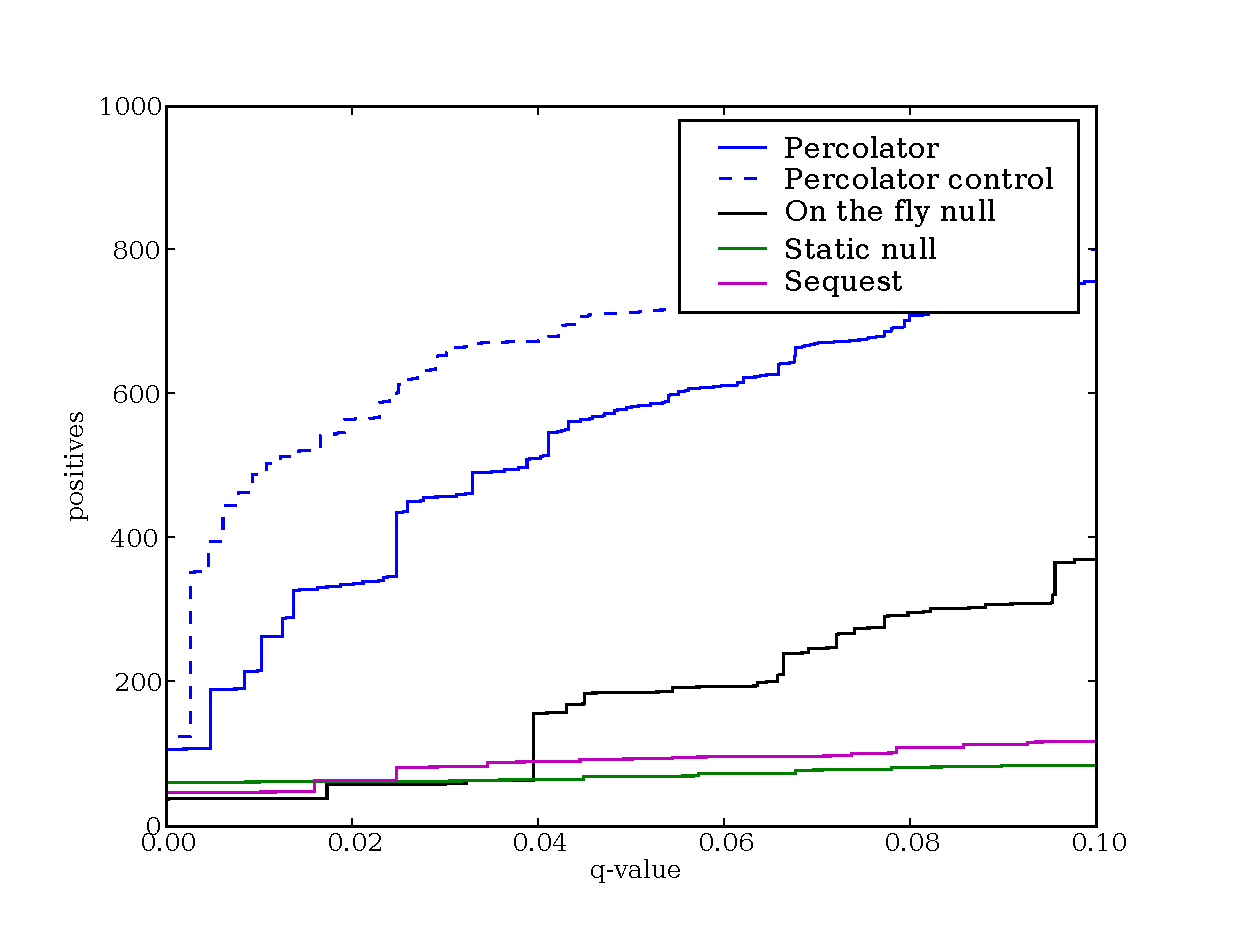
\includegraphics[width=5in]{./Images/q-value.eps}
\caption{{\bf Improved peptide identification.}  The figure plots, for
  a variety of database search algorithms, the number of PSMs as a
  function of the estimated $q$~value.  The five series correspond to
  {\sc Sequest}, Crux's implementation of {\sc Sequest} using a shuffled decoy
  database, Crux using decoys generated on-the-fly, Crux with the
  Percolator post-processor enabled, and Crux with Percolator,
  including retention time features.
  \label{figure:pq-plot}}
\end{figure}

To compare the performance of {\sc Sequest} and the various algorithms
implemented in Crux, we used a collection of FIXME spectra derived
from a yeast whole-cell lysate (see Methods).  Each peptide
identification method searches against the yeast proteome and produces
a list of FIXME PSMs ranked by $q$~value, computed as described in
Section~\ref{section:q-value}.  For SEQUEST and for Crux with a static
decoy database, we use a decoy database of shuffled proteins.
Figure~\ref{figure:pq-plot} plots, for each method, the number of
accepted PSMs as a function of $q$~value threshold.

{\em SEQUEST and Crux get similar results}

{\em Using on-the-fly decoys gets even better results}

{\em Using p-values and percolator get even better results.  It's not
surprising that p-values don't do as well as Percolator, because they
do not take into account many features.  But they are twice as fast.}

\section{Discussion}

The peptide index can be extended to allow for
storage of additional useful pieces of pre-computed information: 
e.g.  predicted peak intensities, predicted peptide retention time,
or peptide proteotypicity.  % probably not a word!

% N.B. We should make sure to mention the file-handle limit at some
% point.

Future work:
\begin{itemize}

\item Estimate PIT

\end{itemize}

\section{Methods}

All experiments were performed on a RedHat Linux machine with an
Athlon MP 2000, 2 x 1.67 GHz processor and 2~GB of RAM.

Using Crux, we precomputed a peptide database for tryptic peptides of
length 6--50 amino acids while allowing missed cleavage sites in the
non-redundant protein database (06/02/2007, 3,292,818 proteins). This
procedure required 19~hours and 14~GB of disk space.

We use the following publicly available tandem mass spectrometry data
sets.  FIXME

\section{Results}

\section*{Acknowledgments}

\section*{Funding}
NIH awards U01~HG003161 and R01~GM071923.

\bibliographystyle{plos}
\bibliography{refs} 

\end{document}
